\section*{ÔN TẬP KIỂM TRA CUỐI KÌ 2 - ĐỀ 05}
\setcounter{ex}{0}\setcounter{bt}{0}
\Opensolutionfile{ans}[ans/ansBTTeX5]

\noindent\textbf{I. PHẦN TRẮC NGHIỆM:}
%Câu 1
\begin{ex}
Giá trị của biểu thức $P=\left(e^2\right)^{\log _e5}$ bằng
\choice
{$\dfrac{1}{5}$}
{$25$}
{$10$}
{$5$}
\end{ex}
%Câu 2
\begin{ex}
Cho hai hàm số $f(x)=a^x$ và $g(x)=\log _ax$. Với $0<a<1$, chọn khẳng định đúng trong các khẳng định sau.
\choice
{$f(x)$ đồng biến và $g(x)$ nghịch biến trên tập xác định}
{$f(x)$ và $g(x)$ nghịch biến trên tập xác định}
{$f(x)$ và $g(x)$ đồng biến trên tập xác định}
{$f(x)$ nghịch biến và $g(x)$ đồng biến trên tập xác định}
\end{ex}
%Câu 3
\begin{ex}
Cho hình chóp $S.ABC$ có $\text{S}A$ vuông góc với mặt phẳng đáy. Góc giữa hai đường thẳng $\text{S}A$ và $BC$ là
\choice
{$60^\circ $.}
{$30^\circ $.}
{$45^\circ $}
{$90^\circ $}
\end{ex}
%Câu 4
\begin{ex}
Cho hình chóp $S.ABCD$ có các cạnh bên bằng nhau và đáy $ABCD$ là hình vuông. Khi đó hình chiếu vuông góc từ $S$ trên mặt phẳng $\left(ABCD\right)$ là
\choice
{Trung điểm cạnh $AB$}
{Tâm đường tròn nội tiếp đáy}
{Trung điểm cạnh $BC$}
{Giao điểm hai đường chéo của $ABCD$}
\end{ex}
%Câu 5
\begin{ex}
Mệnh đề nào sau đây là đúng?
\choice
{Hai mặt phẳng vuông góc với nhau thì mọi đường thẳng nằm trong mặt phẳng này sẽ
vuông góc với mặt phẳng kia}
{Hai mặt phẳng phân biệt cùng vuông góc với một mặt phẳng thì vuông góc với nhau}
{Hai mặt phẳng phân biệt cùng vuông góc với một mặt phẳng thì song song với nhau}
{Hai mặt phẳng vuông góc với nhau thì mọi đường thẳng nằm trong mặt phẳng này và
vuông góc với giao tuyến của hai mặt phẳng sẽ vuông góc với mặt phẳng kia}
\end{ex}
%Câu 6
\begin{ex}
Cho hình hộp chữ nhật $ABCD.A'B'C'D'$. Khẳng định nào sau đây sai?
\choice
{Hình hộp có $6$ mặt là $6$ hình chữ nhật}
{Hai mặt$\left(ACC'A'\right)$ và $\left(BDD'B'\right)$ vuông góc nhau}
{Tồn tại điểm cách đều tám đỉnh của hình hộp}
{Hình hộp có $4$ đường chéo bằng nhau và đồng qui tại trung điểm của mỗi đường}
\end{ex}
%Câu 7
\begin{ex}
Cho hình chóp $S.ABCD$, đáy là hình vuông, có cạnh $SA$ vuông góc với đáy. Khoảng cách từ $S$ đến $(ABCD)$ là
\choice
{$SB$.}
{$BC$.}
{$SC$}
{$SA$}
\end{ex}
%Câu 8
\begin{ex}
Cho hình chóp $S.ABCD$ có đáy là hình vuông, $SA$ vuông góc với đáy. Góc giữa đường thẳng $SC$ và mặt phẳng $(ABCD)$ là:
\choice
{$\widehat{SCB}$}
{$\widehat{CAS}$}
{$\widehat{ASC}$}
{$\widehat{SCA}$}
\end{ex}
%Câu 9
\begin{ex}
Cho hình chóp $S.ABCD$ với đáy $ABCD$ là hình vuông và $SA$ vuông góc với đáy. Góc phẳng nhị diện $\left[S, BD, A\right]$ là góc nào?
\choice
{$\widehat{SOA}$}
{$\widehat{SCA}$}
{$\widehat{SOC}$}
{$\widehat{SAC}$}
\end{ex}
%Câu 10
\begin{ex}
Cho hình chóp $S.ABCD$, đáy $ABCD$ là hình vuông cạnh bằng $a$ và $SA\bot (ABCD)$. Biết $SA=a\sqrt{2}$. Tính góc giữa $SC$ và $(SAB)$.
\choice
{$30^\circ $}
{$45^\circ $}
{$60^\circ $}
{$75^\circ $}
\end{ex}
%Câu 11
\begin{ex}
Một chiếc hộp đựng $15$ cái thẻ giống nhau được đánh số từ $1$ đến $15$. Lấy một thẻ bất kì. Biến cố $A\colon $” Lấy một thẻ ghi số chẵn”, biến cố $B$:” Một thẻ lấy ra ghi số nguyên tố”. Tìm khẳng định sai.
\choice
{$A=\left\{ 2;4;6;8;10;12;14 \right\}$}
{$B=\left\{ 3;5;7;9;11;13 \right\}$}
{$A\cup B\colon$ \lq lq Lấy được một thẻ ghi số chẵn hoặc một thẻ ghi số nguyên tố\rq\rq}
{$B=\left\{ 1;3;5;7;9;11;13 \right\}$}
\end{ex}
%Câu 12
\begin{ex}
Cho $A$, $B$ là hai biến cố xung khắc, $P(A)=0{,}2;P\left(A\cup B\right)=0{,}6$. Tính xác suất của biến cố $B$.
\choice
{$P(B)=0{,}8$.}
{$P(B)=0{,}12$.}
{$P(B)=1{,}2$}
{$P(B)=0{,}4$}
\end{ex}
%Câu 13
\begin{ex}
Đội văn nghệ của lớp 11$A$ có $12$ học sinh trong đó có $7$ em nữ. Cần chọn ra $2$ bạn vào đội văn nghệ của trường. Xác suất để trong $2$ em được chọn có cả nam và nữ là
\choice
{$\dfrac{5}{33}$}
{$\dfrac{7}{22}$}
{$\dfrac{35}{132}$}
{$\dfrac{35}{66}$}
\end{ex}
%Câu 14
\begin{ex}
Tiếp tuyến của đồ thị hàm số $y=x^2$ tại điểm $x_0=1$ có hệ số góc là:
\choice
{$1$}
{$2$}
{$-2$}
{$-1$}
\end{ex}
%Câu 15
\begin{ex}
Cho $u=u(x);v=v(x)$ là các hàm số có đạo hàm tại điểm $x$ thuộc khoảng xác định; $k$ là số thực tùy ý. Chọn khẳng định đúng.
\choice
{$(u+v)'=u'+v'$}
{$(uv)'=u' \cdot v'$}
{$\left(\dfrac{u}{v}\right)'=\dfrac{u'}{v'}$}
{$\left(k \cdot u\right)'=k' \cdot u'$}
\end{ex}
%Câu 16
\begin{ex}
Cho hàm số $f(x)=x^3+3x^2+1$. Tính $f''(x)$.
\choice
{$f''(x)=3x^4+6x^3$}
{$f''(x)=12x^5+18x^4$}
{$f''(x)=3x^2+6x$}
{$f''(x)=6x+6$}
\end{ex}
%Câu 17
\begin{ex}
Cho hai số thực dương $a,b$. Rút gọn biểu thức $A=\dfrac{a^{\tfrac{1}{4}}\sqrt[3]{b}+{b^{\tfrac{1}{4}}}\sqrt[3]{a}}{\sqrt[12]{a}+\sqrt[12]{b}}={a^{\tfrac{1}{m}}} \cdot {b^{\tfrac{1}{n}}}$. Tính $P=\dfrac{m}{n}$?
\choice
{$P=\dfrac{1}{2}$}
{$P=0$}
{$P=8$}
{$P=1$}
\end{ex}
%Câu 18
\begin{ex}
Cho $a,b$ là các số thực dương và $a$ khác $1$, thỏa mãn ${\log_{a^3}}\dfrac{a^5}{\sqrt[4]{b}}=2$. Giá trị của biểu thức $\log _ab$ bằng:
\choice
{$4$}
{$-4$}
{$-\dfrac{1}{4}$}
{$\dfrac{1}{4}$}
\end{ex}
%Câu 19
\begin{ex}
\immini{Từ các đồ thị $y=\log _ax$, $y=\log _bx$, $y=\log _cx$ đã cho ở hình vẽ. Khẳng định nào sau đây đúng?
\choice
{$0<a<b<1<c$}
{$0<c<1<a<b$}
{$0<c<a<1<b$}
{$0<c<1<b<a$}
}{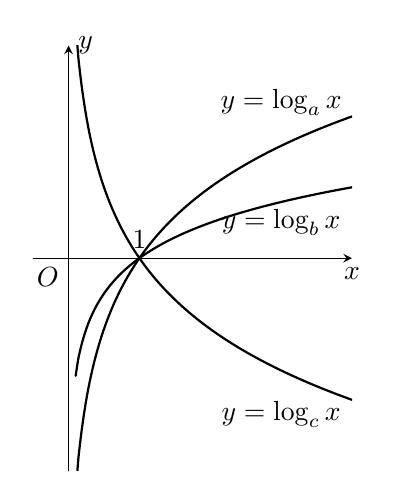
\begin{tikzpicture}[line join = round, line cap = round, >=stealth, scale = .9]
%Hệ trục Oxy và hàm số cần vẽ
\def\xmin{-.5}     \def\xmax{4}
\def\ymin{-3}       \def\ymax{3}
\def\f(#1){ln(#1)/ln(4)}
\def\g(#1){ln(#1)/ln(2)}
\def\h(#1){ln(#1)/ln(0.5)}
%Vẽ hệ trục
\draw[->] (\xmin,0)--(0,0) node[below left]{$O$}--(\xmax,0) node[below]{$x$};
\draw[->] (0,\ymin)--(0,\ymax) node[right]{$y$};
\draw (1,0)node[above]{$1$} (3,2.2)node{$y=\log_ax$} (3,0.5)node{$y=\log_bx$} (3,-2.2)node{$y=\log_cx$};
%Vẽ hàm số
\begin{scope}
\clip (\xmin,\ymin) rectangle (\xmax,\ymax);
\draw[smooth, thick, black] plot[domain = 0.1:\xmax, samples = 200, variable=\x]({\x},{\f(\x)});
\draw[smooth, thick, black] plot[domain = 0.1:\xmax, samples = 200, variable=\x]({\x},{\g(\x)});
\draw[smooth, thick, black] plot[domain = 0.1:\xmax, samples = 200, variable=\x]({\x},{\h(\x)});
\end{scope}
\end{tikzpicture}
}
\end{ex}
%Câu 20
\begin{ex}
Tìm tích số của tất cả các nghiệm thực của phương trình ${7^{x^2-x+\dfrac{3}{2}}}=49\sqrt{7}$.
\choice
{$-1$}
{$1$}
{$-\dfrac{1}{2}$}
{$\dfrac{1}{2}$}
\end{ex}
%Câu 21
\begin{ex}
Tập nghiệm của bất phương trình $2\log _2(x-1)\le \log _2(5-x)+1$ là
\choice
{$[3;5]$}
{$(1;3]$}
{$[1;3]$}
{$(1;5)$}
\end{ex}
%Câu 22
\begin{ex}
Khẳng định nào sau đây sai?
\choice
{Nếu đường thẳng $d$ vuông góc với hai đường thẳng cắt nhau nằm trong $\left(\alpha\right)$ thì $d$ vuông góc với bất kì đường thẳng nào nằm trong $\left(\alpha\right)$}
{Nếu đường thẳng $d\bot \left(\alpha\right)$ thì $d$ vuông góc với mọi đường thẳng trong $\left(\alpha\right)$}
{Nếu đường thẳng $d$ vuông góc với hai đường thẳng nằm trong $\left(\alpha\right)$ thì $d\bot \left(\alpha\right)$}
{Nếu $d\bot \left(\alpha\right)$ và đường thẳng $a//\left(\alpha\right)$ thì $d\bot a$}
\end{ex}
%Câu 23
\begin{ex}
Cho hình chóp $S.ABCD$ có đáy là hình thoi cạnh $a$, $SA=SB=SC=\dfrac{2a}{3}$, $\widehat{ABC}=60^\circ$. Tính góc giữa hai mặt phẳng $(SCD)$ và $(ABCD)$.
\choice
{${{30}^\circ}$.}
{${{45}^\circ}$.}
{${{90}^\circ}$}
{${{60}^\circ}$}
\end{ex}
%Câu 24
\begin{ex}
Cho hình chóp đều $S.ABCD$ có $AB=a;SA=a\sqrt{2}$. Tính góc giữa $SC$ và mặt phẳng đáy.
\choice
{${{30}^\circ}$}
{${{45}^\circ}$}
{${{90}^\circ}$}
{${{60}^\circ}$}
\end{ex}
%Câu 25
\begin{ex}
Cho hình chóp tứ giác đều $S.ABCD$ có cạnh đáy bằng $a$ và chiều cao bằng $a\sqrt{2}$. Khoảng cách từ $AB$ đến mặt phẳng $(SCD)$ bằng
\choice
{$\dfrac{2a\sqrt{6}}{3}$}
{$\dfrac{3a\sqrt{2}}{2}$}
{$a\sqrt{6}$}
{$a\sqrt{3}$}
\end{ex}
%Câu 26
\begin{ex}
Cho hình chóp $S.ABCD$ có $SA\bot (ABCD)$, đáy $ABCD$ là hình vuông có cạnh bằng $a$, $SA=a\sqrt{3}$. Số đo của góc nhị diện $\left[B, SA, C\right]$ bằng
\choice
{${{30}^\circ}$}
{${{45}^\circ}$}
{${{60}^\circ}$}
{${{90}^\circ}$}
\end{ex}
%Câu 27
\begin{ex}
Cho hình lăng trụ đứng $ABC. A'B'C'$ có $\triangle ABC$ đều cạnh $a,AA'=\sqrt{3}a$. Góc giữa đường thẳng $AB'$ và $(ABC)$ bằng
\choice
{${{45}^\circ}$}
{${{90}^\circ}$}
{${{30}^\circ}$}
{${{60}^\circ}$}
\end{ex}
%Câu 28
\begin{ex}
Cho hàm số $f(x)=\dfrac{x+3}{x+1}$ có đồ thị $(C)$. Phương trình tiếp tuyến của đồ thị $(C)$ tại giao điểm của đồ thị với trục $Oy$ là
\choice
{$2x-y-3=0$}
{$2x+y+3=0$}
{$2x-y+3=0$}
{$2x+y-3=0$}
\end{ex}
%Câu 29
\begin{ex}
Đạo hàm của hàm số $y={{10}^{x^2}}$ là
\choice
{${{10}^{x^2}} \cdot \ln 10$}
{$2x \cdot 10^{x^2}$}
{$2x \cdot 10^{x^2} \cdot \ln 10$}
{$\dfrac{1}{2}+\log_2 10$}
\end{ex}
%Câu 30
\begin{ex}
Cho hàm số $f(x)=\dfrac{2mx-3}{x+1}\,\left(m\in \mathbb{R},m\ne -\dfrac{3}{2}\right)$. Gọi $S$ là tập các giá trị của $m$ để $f'(0) \cdot f'(-2)=4$. Tổng các phần tử của $S$ bằng:
\choice
{$4$}
{$\dfrac{5}{4}$}
{$2$}
{$-3$}
\end{ex}
%Câu 31
\begin{ex}
Cho hàm số $f(x)=\sqrt{2x^2+2x+a^2+3}$. Gọi $S$ là tập các giá trị của $a$ để $f'(1)=1$. Tích các phần tử của $S$ bằng:
\choice
{$4$}
{$2\sqrt{2}$}
{$2$}
{$-\,2$}
\end{ex}
%Câu 32
\begin{ex}
Hai xạ thủ bắn vào bia một cách độc lập với nhau, mỗi người bắn một viên đạn. Xác suất băn trúng bia của hai xạ thủ lần lượt là $\dfrac{1}{3}$ và $\dfrac{1}{5}$. Tính xác suất của biến cố “có ít nhất một xạ thủ không bắn trúng bia”.
\choice
{$\dfrac{14}{15}$}
{$\dfrac{1}{15}$}
{$\dfrac{8}{15}$}
{$\dfrac{1}{3}$}
\end{ex}
%Câu 33
\begin{ex}
Trong một thùng có $40$ tấm thẻ được đánh số thứ tự từ $1$ đến $40$. Người ta rút ra từ thùng phiếu một tấm thẻ bất kì. Tính xác suất của biến cố “ tấm thẻ rút được có số thứ tự chia hết cho $4$ hoặc $5$”
\choice
{$\dfrac{1}{2}$}
{$\dfrac{1}{3}$}
{$\dfrac{2}{5}$}
{$\dfrac{9}{20}$}
\end{ex}
%Câu 34
\begin{ex}
Lớp 12A có $32\%$ học sinh giỏi môn Toán, $28\%$ học sinh giỏi môn Văn và $20\%$ học sinh học giỏi cả hai môn Toán và Văn. Chọn ngẫu nhiên một học sinh của lớp 12A. Xác suất để chọn được một học sinh không giỏi môn nào trong hai môn Toán, Văn là?
\choice
{$0{,}35$}
{$0{,}42$}
{$0{,}5$}
{$0{,}6$}
\end{ex}
%Câu 35
\begin{ex}
Trên đường từ nhà bạn Tuấn đến trường có ba vị trí có đèn tín hiệu giao thông. Biết xác suất gặp đèn đỏ tại ba vị trí đó lần lượt là $x$, $y$ và $0{,}5$ (với $x>y$). Biết xác suất để ít nhất một trong ba vị trí gặp đèn đỏ là $0{,}79$ và xác suất để cả ba vị trí gặp đèn đỏ là $0{,}06$. Xác suất để có đúng hai vị trí gặp đèn đỏ là
\choice
{$0{,}29$}
{$0{,}27$}
{$0{,}3$}
{$0{,}26$}
\end{ex}

\noindent\textbf{II. PHẦN TỰ LUẬN}
%Câu 36 
\begin{ex}
Giải phương trình $\log_{\sqrt{3}}\left( x-2 \right)+\log_{3} \left( x-4 \right)^{2}=0$
\end{ex}
%Câu 37
\begin{ex}
Viết phương trình tiếp tuyến đồ thị hàm số $y=x^4-x^2+1$ tại giao điểm với trục tung.
\end{ex}
%Câu 38
\begin{ex}
Một chiếc máy có hai động cơ I và II hoạt động độc lập với nhau. Xác suất để động cơ I và động cơ II bị hỏng lần lượt là $0.05$ và $0.02$. Tính xác suất để có ít nhất một động cơ chạy tốt.
\end{ex}
%Câu 39
\begin{ex}
Cho khối lăng trụ $ABC \cdot A'B'C'$ có đáy là tam giác vuông cân tại $A$, $A'A=A'B=A'C=a$. Biết góc giữa hai mặt phẳng $\left(BCC'B'\right)$ và $(ABC)$ bằng $30^\circ $. Tính thể tích của khối lăng trụ đã cho.
\end{ex}


\Closesolutionfile{ans}